\chapter{Implementation}
\label{chapter:implementation}

This chapter addresses the main decisions taken in order to implement the hardware and software architectures presented in Chapter 3.


\section{Hardware Architecture}


The next sections provide the implementation choices for the hardware architecture described in Chapter \ref{chapter:architecture}. As shown in Figure~\ref{architecture_system} we require tablet to run the HUB app, HVAC control, lighting control and a \ac{BLE} beacon for user location tracking.



\begin{figure}[h]
\centering
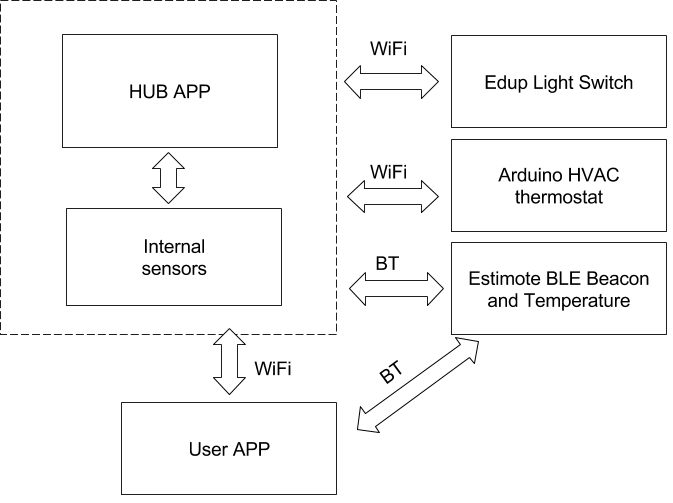
\includegraphics[width=0.7\textwidth]{Figures/top_view}
\caption{Architecture of the system}
\label{architecture_system}
\end{figure}





%This chapter is divided in three main sections. In Section 4.1 the detailed hardware architecture is
%described. Each of its subsection shows the decisions taken in the selection of the components.
%Section 4.2 describes the implementation of the software architecture. This section is composed of
%several subsections that detail the software configuration and explains the developed code.
%Finally, Section 3.5 details the deployment of the system in a set of offices at IST - Taguspark.

\subsection{Tablet}

A tablet capable of supporting a range of communication protocols and with some embedded sensors must be chosen as the base for the solution.

Several tablets were taken in consideration, the decisive factors were the price, \ac{CPU} speed/cores, \ac{RAM} and finally the supported communication protocols (\ac{BLE} and \ac{WiFi} are required). These factors are important since they allow the device to easier bought (price), allow multiple parallel complex computational operations like image processing, video recording, voice recognition (\ac{CPU} speed/cores and \ac{RAM}), devices with lower \ac{CPU} and \ac{RAM} may produce unexpected and unwanted results like crashes due to lack of resources. Since the device will be communication with a client device as talked about in section XXX (user app link......) it requires \ac{WiFi} to transfer and receive data and commands, \ac{BLE} can be used to receive external sensor data such as temperature.


Table~\ref{table:tablet} shows some examples of tablets running the major operating systems with similar hardware specifications.

In terms of price Apple tablets have the largest cost, since there is such a big gap in cost the iPad Mini 4 does not fit our needs. There are many types of Windows and Android tablets with very affordable prices. The Nexus was chosen because it was developed by Google in partnership with Asus, has very good reviews and is updated to the latest android version. There are Windows tablets cheaper than the HP ENVY 8 sold by Microsoft but there were a lack of reviews so a good tablet from a big manufacturer was picked.

The Android and Windows tablets have very similar hardware specifications. So the tablet chosen was the Nexus 7 (2013) since the programmer had previously developed Android apps.


\begin{table}[]
\centering
\begin{tabular}{|l|l|l|l|l|}
\hline
\textbf{name} & \begin{tabular}[c]{@{}l@{}}Apple iPad \\ mini 4\end{tabular} & Nexus 7 2013 & \begin{tabular}[c]{@{}l@{}}HP ENVY \\ 8 Note 5009\end{tabular} \\ \hline
\textbf{CPU speed} & 1.5 GHz & 1.5 GHz & 1.44 GHz \\ \hline
\textbf{CPU cores} & 2 & 4 & 4 \\ \hline
\textbf{RAM} & 2GB & 2GB & 2GB \\ \hline
\textbf{WiFi} & \begin{tabular}[c]{@{}l@{}}yes (2.4 GHz \\ and 5 GHz)\end{tabular} & \begin{tabular}[c]{@{}l@{}}yes (2.4 GHz \\ and 5 GHz)\end{tabular} & yes (2.4 GHz) \\ \hline
\textbf{BLE} & yes & yes & yes \\ \hline
\textbf{Light sensor} & yes & yes & yes \\ \hline
\textbf{Microfone} & yes & yes & yes \\ \hline
\textbf{Speaker} & yes & yes & yes \\ \hline
\textbf{Front camera} & yes & yes & yes \\ \hline
\textbf{Size} & \begin{tabular}[c]{@{}l@{}}7.9 inches (1536 \\ x 2048 pixels)\end{tabular} & \begin{tabular}[c]{@{}l@{}}7 inches (1200 \\ x 1920 pixels)\end{tabular} & \begin{tabular}[c]{@{}l@{}}8 inches (1200 \\ x 1920 pixels)\end{tabular} \\ \hline
\textbf{Operating System} & Apple IOS 10.0.1 & Android 6.0 & Windows 10 \\ \hline
\textbf{Cost (EUR)} & 449 & 131 & 178 \\ \hline
\end{tabular}
\caption{Comparison between some tablet devices}
\label{table:tablet}
\end{table}


\subsection{HVAC control}
In order for our \ac{BAS} solution to control an \ac{HVAC} system we would need to either communicate with a building central controlling unit or physically controlling the system like a thermostat does. Since many buildings don't have a central control point running some kind of server where you can control it using the internet, we went with the thermostat route.

For our smart thermostat to work we require a device capable of sending electric impulses to the \ac{HVAC} wire. 

Table~\ref{thermostat-choice} shows some commercial products and a Arduino solution.

We require a device that offers a  API in order to be controlled by our tablet, because the Sensi thermostat does not offer an official API it does not fit our requirements.

The Nest thermostat is the most popular option in the market integrated in many home automation systems, but since one of our requirements is keeping the cost low it does not fit our requirements. The path chosen was developing an Arduino solution with built in \ac{WiFi}, a relay to control the electric wires and a temperature and humidity sensor.



\begin{table}[]
\centering
\begin{tabular}{|l|l|l|l|}
\hline
\textbf{Name} & \begin{tabular}[c]{@{}l@{}}Sensi Wi-Fi \\ Thermostat\end{tabular} & \begin{tabular}[c]{@{}l@{}}Nest (3rd)\\ Thermostat\end{tabular} & \begin{tabular}[c]{@{}l@{}}Wemos D1 \\ mini Arduino + \\ Temperature Humidity \\ Sensor DHT11 + \\ Solid State Relay \\ 4 Channel + box\end{tabular} \\ \hline
\textbf{temperature/humidity} & yes & yes & yes \\ \hline
\textbf{Developer API} & no & yes & yes \\ \hline
\textbf{Cost (EUR)} & 116 & 223 & 4 + 1.5 + 6 + 1 = 12.5 \\ \hline
\end{tabular}
\caption{Differences between thermostat options.}
\label{thermostat-choice}
\end{table}


\subsection{Lighting control}
Besides controlling the room \ac{HVAC}, we require control over the lighting system. After some research we had three options: using wireless controllable light bulbs, using some kind of Arduino/relay solution like the thermostat or using a wireless controllable light switch.

Table~\ref{lighting-choice} show some available options.

Our lighting solution should be affordable, allow touch control and control using an API. The Philips Hue is costly and does not have lights supported by our office (fluorescent tube lamp) for these reasons it does not fit our requirements.

In order for our solution to be easily deplorable it requires the least amount of assembly and soldering components, an pre-built lighting product is preferable if the price range is close enough. Both the Arduino/relay and the DI-O/Arduino options have shortcomings, the first does not provide touch control and requires soldering and the latter also requires soldering in the Arduino interface side.

The lighting option chosen was the Edup Smart Light Switch, it provides touch control of the lighting, supports any existing infrastructure in existing buildings and is not too expensive.


Originally in Section \ref{architecture3} of the architecture, the lighting system was going to be integrated with the Arduino/\ac{HVAC} using relay actuators. We decided go with the Edup light switch after more searching for lighting products we could control, it is a better solution because of the touch control and no need for assembly as described previously.

\begin{table}[]
\centering
\begin{tabular}{|l|l|l|l|l|}
\hline
\textbf{Name} & \begin{tabular}[c]{@{}l@{}}Edup  - Wireless \\ Smart Home Wifi \\ Lighting Power\\ Switch\end{tabular} & \begin{tabular}[c]{@{}l@{}}Philips Hue Bridge + \\ light bulb +\\  light switch\end{tabular} & \begin{tabular}[c]{@{}l@{}}Wemos D1 \\ mini Arduino +  \\ Solid State Relay \\ 4 Channel + box\end{tabular} & \begin{tabular}[c]{@{}l@{}}DI-O - light \\ module + \\ DI-O double \\ light switch + \\ Wemos D1 \\ mini Arduino +\\  RF Transmitter \\ Receiver Module \\ 433MHz + box\end{tabular} \\ \hline
\textbf{manual control} & yes & yes & no & yes \\ \hline
\textbf{Developer API} & yes  (not officialy) & yes & yes & yes (arduino) \\ \hline
Wifi & yes & yes & yes & \begin{tabular}[c]{@{}l@{}}yes (needs arduino \\ to interface with \\ RF signals)\end{tabular} \\ \hline
\begin{tabular}[c]{@{}l@{}}Already built\\ (no extra work)\end{tabular} & yes & yes & no & \begin{tabular}[c]{@{}l@{}}no (needs arduino \\ and RF components \\ to be built)\end{tabular} \\ \hline
\begin{tabular}[c]{@{}l@{}}Support for \\ any office \\ (any light bulb)\end{tabular} & yes & no & yes & yes \\ \hline
\textbf{Cost (EUR)} & 27.93 & 56,31 +39,34 = 95,65 & 4 + 6 + 1 = 11 & \begin{tabular}[c]{@{}l@{}}18,40 + 24,40 + 4 \\ + 0,5 +1 = 48,3\end{tabular} \\ \hline
\end{tabular}
\caption{Lighting control options.}
\label{lighting-choice}
\end{table}


\subsection{Bluetooth Beacon}

We require a way to determine if a user is near a certain point in the building such as the office. In section XXX this will be approach in higher detail.

From the alternatives seen in Section~\ref{ocupacy_detection}, we  determined that \ac{BLE} beacons an option to achieve room base location in a building.

There are many kinds of devices capable of emitting \ac{BLE} packets: android devices( available in version 5.0), some microcontrolers and commercial beacon products.

We decided to use a Estimote beacon, the reason it was chosen was because we had one extra around. Since it is portable we can position it anywhere in the room, enabling better coverage, as it does not need to be connected to a power socket.








\section{Software Architecture}

\subsection{HUB APP}

\begin{figure}[h]
\centering
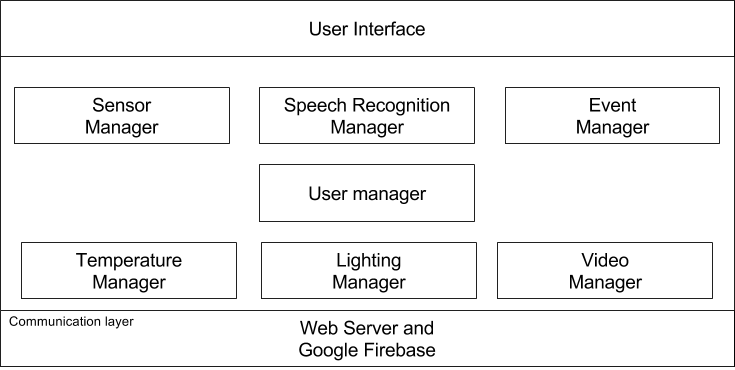
\includegraphics[width=0.7\textwidth]{Figures/software_implementation}
\caption{Software architecture of HUB APP}
\label{software_imp}
\end{figure}

There were a couple of changes in regard to the starting software architecture, we will present the current implementation:

\subsubsection{Event Manager}\mbox{}\\

The Event Manager  operates in a publish/subscriber basis. Other managers register their interest in certain events and when whose events happen they are notified. The events can be published to the event manager by any other manager. For example the Sensor Manager can publish and motion detected event, that the video manager is interested.

Currently there are eight different events available:

\begin{itemize}
  \item \textbf{Temperature:} Contain the current temperature and humidity.
  \item \textbf{Motion:} This event contains a boolean to inform if movement is detected, and long value with the time since last movement was detected.
  \item \textbf{Speech:} The phrase of an successful speech recognition.  
  \item \textbf{Time:} If we need to check some task regularly this event is triggered every 2 seconds.  
  \item \textbf{User location:} This event contains the user id, the location type (Office/Building), a boolean to specify if he is in the location or left and finnaly a boolean.
  \item \textbf{Brightness:} The value in Lux of the light sensor.  
  \item \textbf{Light:} The light number and it's status. 
  \item \textbf{Change temperature:} The value of temperature we want the thermostat to be at. 
  
\end{itemize}


The Event Manager also receives a list a recipes created by the user. These recipes contain a list a trigger and actions. When a event is published all the recipes are examined to see if all triggers conditions are fulfilled. When this happens all the actions in that particular recipe are executed.

There are six triggers available:

\begin{itemize}
  \item \textbf{Temperature:} This trigger allows the user to trigger an action when the office temperature is bellow or above a value specified.
  \item \textbf{Motion:} The motion sensor is triggered when something changes in the field of view of the assistant or no movement detected in X seconds.
  \item \textbf{Speech:} Say the keyword "my assistant" and after the beep you say the phrase specified in the trigger.  
  \item \textbf{Time:} The timer trigger allows the user to run certain actions at a specific time(Scheduler).  
  \item \textbf{User location:} Allows the user to choose from a list of different scenarios ("User is inside office", "User is inside building", "User leaves office", "User leaves building", "User arrives at office", "No user inside building", "No user inside office" and "User arrives at building").
  \item \textbf{Light sensor:} The light sensor triggers an action if the light level is bellow or above the value specified.
  
\end{itemize}

The actions available are:

\begin{itemize}
  \item \textbf{Light:} Sets the state of the lights.
  \item \textbf{Temperature:} Changes the target temperature and turns on the HVAC if needed.
  \item \textbf{Speech:} This action uses the speakers to say the text specified (text to speech).
\end{itemize}


\subsubsection{Speech Recognition Manager}\mbox{}\\

This manager uses the CMU Sphinx offline keyword speech recognizer, meaning it will detect one word in our case "my assistant". When it detects the keyword it shuts down and we launch google online speech recognition. We use this other speech recognition because it offer good results, the reason the manager uses two different speech recognizes is because using only google recognizer has higher bandwidth cost since we would be constantly sending audio.The other reason is privacy, we don't know if google is going to disclose our audio files to third parties.

When we successfully say the keyword a beep sound is played and google speech recognizer listens to the rest of the voice command, when the results arrive from google they are published to the Event manager.

There were several problems with both recognizer, the Sphinx has a lot of false positives for small words, for our current keyword we sometimes need to repeat more than once for it to recognize. This problem can perhaps be attributed to the fact we are not native English speakers. 
Google speech recognizer is plagued with problems since a few version ago, it sometimes will not listen and shutdown after some 100 ms. To try to minimize the problem by run a check every 10 seconds. If both speech recognizes are not running we relaunch Sphinx.

\subsubsection{Sensor Manager}\mbox{}\\

The Sensor Manager is responsible for the light sensor and virtual motion sensor.

The light sensor is built in in the tablet. Every 2 seconds the current light level is published to the Event manager. 

Since the tablet does not have a motion sensor, we use the front camera and analyze the frames every second. If the total number of the RGB pixels with threshold above 50 is different we know there was a change in the eye sight of the camera. The percentage of different pixels for a positive detection is user defined, the default is 0.5%.

A problem that motion detecting cameras have are the false positives specially when there is a windows to the outside. A strong light can trigger the sensor, because of that we designed the sensor be able to ignore an area of the camera frame. It is possible to specify the area to ignore in the HUB APP settings.


\subsubsection{Video Manager}\mbox{}\\

The Video manager does two jobs, it records 30 seconds videos when no user is present in the office and motion is detected. The other job is offering a live preview of the office, an user can use the USER APP to watch in real time the office.

The recorded videos don't have any audio because Android does not allow the audio to be shared between the speech recognizer and the video recorder at the same time.

The video manager can be enabled and disabled in the HUB settings for privacy reasons.



\subsubsection{Lighting Manager}\mbox{}\\

This manager is responsible for turning on/off the room lights and keeping their status updated when a user uses the manual switch.


The lights in the room are controlled by the Edup Light Switch, the switch must be connected to a WiFi network and automatically establishes a connection to Edup servers to enable remote control over the switch.

In order for our app to control the light switch we must send a byte array with the data shown in Figure~\ref{edup_imp}.
The message starts and ends with specific hex strings, the middle part of the message seems to always start with "ZH03", followed by the light switch id then a 1 and finally the lights sate we want to change. For example if the ending part of the middle message is "101" then the first and last lights will be turned on, and the middle one turned off.

At this point we achieved control over the lights, but since there is a physical light switch interface we must update our application status if a button is pressed outside our app.
The Edup Light Switch sends a \ac{UDP} multicast message when the lights are changed. A \ac{UDP} server was implemented, when any message was received its content is verified in order to determine if it is a Edup Light switch message. The message must start with "7e7e000d0002" and end with "7f7f". The middle text is "1101", the first character is always the same and the three other represent the current status of the lights.

There were some difficulties since there is no official API. In order to understand how the light switch worked, we used Wireshark to sniff the connection and try to replicate the messages.

One other problem arised when we quickly turned on/off all the lights in quick succession. When we turn off the first light at the app the light switch sends the multicast message to notify the network, but if we have already turned off the second light then by the time the \ac{UDP} multicast message arrives the state is already different and some lights my turn on back again. To fix this problem when a light is pressed in the app we ignore any \ac{UDP} message for 3 seconds.



\begin{figure}[h]
\centering
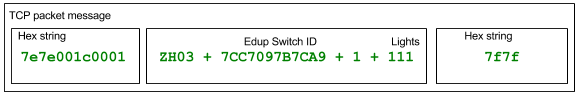
\includegraphics[width=0.8\textwidth]{Figures/Edup_imp}
\caption{Edup packet to set the light state.}
\label{edup_imp}
\end{figure}


\subsubsection{Temperature Manager}\mbox{}\\


The Temperature Manager is responsible for keeping an updated weather forecast, keeping an updated temperature reading and turning on/off the Arduino \ac{HVAC}.

The forecast uses wunderground service API and is used to give information to the user about the current weather conditions.

There are two different configurations to access the temperature in our solution, using an Estimote beacon or the Arduino \ac{HVAC}. 
The beacon sends a Eddystone telemetry packet containing the current temperature, it is intended for situations when we just want to display the temperature.
The Arduino option gives the temperature and humidity and allows us to control the \ac{HVAC} system.


In order to obtain the beacon temperature, it must be configured to the Eddystone-UID primary packet type using the Estimote mobile app. Then the beacon id must be set in the HUB APP settings.

To get temperature readings from the Arduino \ac{HVAC} and we do a \ac{HTTP}  GET request to the Arduino device IP address at the "/data" endpoint. We receive a \ac{JSON} message containing the temperature/humidity. There is a discovery mechanism to setup the Arduino location it will be mentioned in detail later.

To turn on/off the \ac{HVAC} we send send a POST request containing a \ac{JSON} message containing the relay channels we want to turn on/off. In Figure~\ref{arduino_post_imp} the channel configuration is shown. If we want cold air we set the "ch1" to 1 and "ch3" to 1, the other channels must be set o zero ,the \ac{HVAC} starts sending cold air at slow speed.


\begin{figure}[h]
\centering
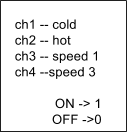
\includegraphics[width=0.3\textwidth]{Figures/temperature_post_imp}
\caption{Arduino HVAC configuration.}
\label{arduino_post_imp}
\end{figure}


\subsubsection{User Manager}\mbox{}\\


The User Manager keeps track of the user location (in building, in office) and is responsible for registering new users.

The location system works in the following simplified manner, it receives two types of location messages in-building or in-office, there are timeouts in place so in the eventuality that no message is received for a certain amount of time we assume the user has left the office or building. The in-building messages arrive every 60 seconds and in-office every 1 second, the timeouts are 120 seconds and 20 seconds respectively.

Since the location is mainly done in the USER APP, it will be explained in detail later.


There are two types of user that can register. Users with the mobile USER APP and users without it. If a user has the app, it just needs to open the app and there is an semi-automatic register process. If the user does not have the app he will receive an email with an QR-Code that will act as an identification card, when the user places the card in front of the HUB camera he is logged on for a certain amount of minutes specified by the user. Since we can't track the user whereabouts without the app, the user will have to manually turn the lights and \ac{HVAC} if he leaves while logged on.



\subsubsection{Web Server and Google Firebase}\mbox{}\\

These independent modules are responsible for communication with the USER APP.

The HUB runs a JAVA Spark server at port 5002 and offer an \ac{JSON} API.

\begin{itemize}
  \item \textbf{GET /register:} Returns the HUB UUID, description and name.
  \item \textbf{POST /register:} Receives the name, email and UUID of a new user. Returns a status true/false depending if the registration was successful.
  \item \textbf{POST /location} Receives an UserLocation object, Figure~\ref{user_location_class}.
  \item \textbf{POST /make-changes:} Receives the temperature value we want "targetTemperature", and receives an boolean array representing the lights we want to change "lightsState";
   \item \textbf{GET /status:} Returns the current temperature and a boolean array representing the lights.
   \item \textbf{GET /alive:} Returns a status "true" signifying the server is running.
\end{itemize}






\begin{figure}[h]
\centering
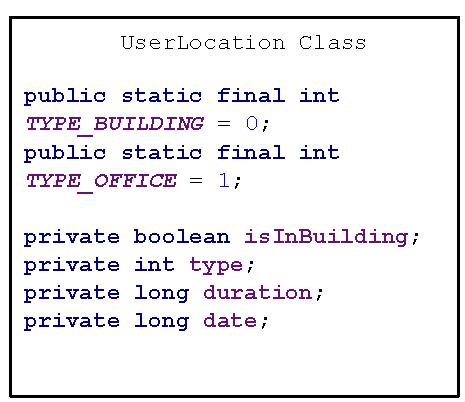
\includegraphics[width=0.4\textwidth]{Figures/userlocation_class}
\caption{UserLocation Class parameters.}
\label{user_location_class}
\end{figure}



Originally the plan was to only use the web server, but in our building we can't run web servers in the WiFi network. When we tried to contact the HUB it did not receive any request, then we changed to a private wireless network it all worked normally.

The solution we found was Google Firebase, it is a platform that offers multiple services. We use two services, the real-time database and the storage.
The database allows us to store and sync data in a NoSQL cloud database. Using an Android library developed by them we can store JAVA objects directly to the database. The storage service is used to upload the recorded videos and live preview images, captured by the Video Manager.

Firebase solves us two problems, one is users can access our solution from their home and access the live camera, it uses firebase as a middle man to communicate. The second problem it fixed was the user location tracking, since our building is big, the private network where the tablet is connected can't be access in most of the building. A user entering the building could not communicate with our HUB and notify of it's presence since they were in different networks, we use Firebase to add our location messages that are then received by the HUB and building location is achieved.

We ended having two ways to communicate with the HUB APP, each has some strong and weak points. 

The negative points with Firebase are it requires internet to work so we had to keep the web server in order for our solution to work inside the office even when no internet connectivity was present. One other problem is the free tear only allows 100 simultaneous connections, which means there can only be a maximum of 100 users and HUB devices connect at each moment.

One weak point of the web server is it's response time varies a lot, some times just a few milliseconds up to a few seconds for simple static content. The server is running in a separate thread but while the APP is in the foreground the response times increase a bit.



\subsubsection{User interface}


The \ac{UI} of the HUB APP is composed of three main screens. There are a lighting screen, a temperature and general menu that contains several advanced features.

The \textbf{lighting screen}, shown in Figure~\ref{screen_lights} allows the user to control the lighting environment in the room.

The \textbf{temperature screen}, shown in Figure~\ref{screen_temperature} gives visual information about the current weather outside. There is also a virtual thermostat where the user can select the temperature he desires. The thermostat shows a leaf icon when the selected temperature is inside the range of temperature where most people have comfort as described in section~\ref{related:adaptive_heating}. 

There is a \textbf{general menu} that contains the other screens that enable additional features. This menu contains:
\begin{itemize}
  \item \textbf{User registration:} Allows the a person to setup an account in HUB. 
  \item \textbf{Recipe management:} Contains a list of the current recipes in the HUB and allows the user to create, edit, disable/enable and delete them.
  
  \item \textbf{Event history} Shows a list events ordered chronologically. 
  
  \item \textbf{Statistics screen} Shows temperature, lighting and occupation graphs. 
  
  \item \textbf{Settings screen} Allows the user to configure the HUB APP.
\end{itemize}



The \textbf{user registration screen} allows the user to register using the USER APP or an email address.
If the user uses the Android USER APP to register, a visual registration token is shown in the form of a QR-Code. The QR-Code contains a temporary id and the IP address of the HUB server. This temporary id is latter needed when the user registers and exists  only to ensure only people inside the office can register a new user and not just anyone that knows the IP address.

In the \textbf{recipe screen}, the user can create new recipes, first the trigger/s is selected, only then can the action/s be picked. In Figures \ref{create_recipe}, \ref{screen_triggers}, \ref{screen_actions} and \ref{screen_completed_recipe} the steps needed to create a recipe are shown, the resulting recipe turns on all the room lights if a user is inside the office and the light level is low. 

The \textbf{settings screen}, (falar do kiosk e de todas as opçoes)





\begin{figure}[h]
\centering
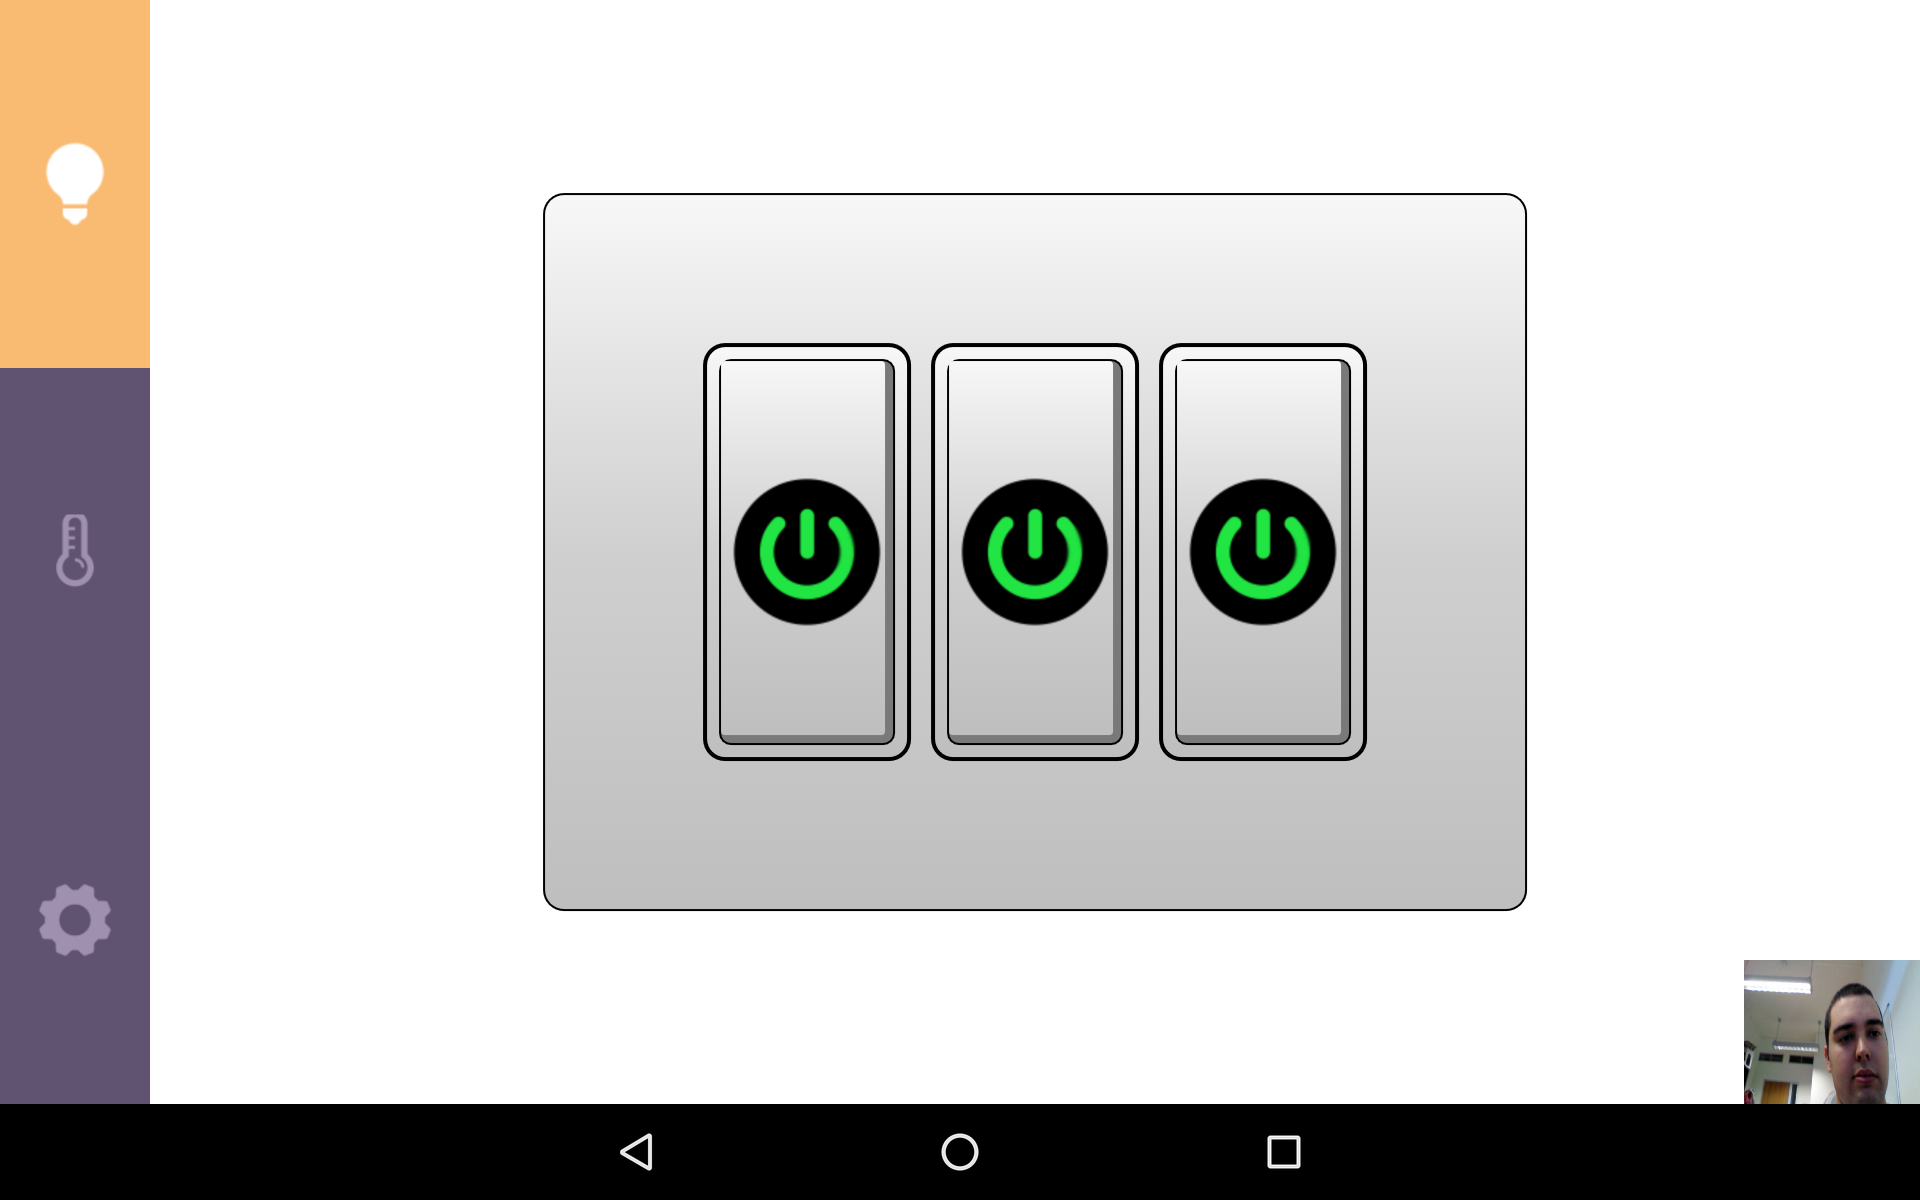
\includegraphics[width=0.7\textwidth]{Figures/screen_lights}
\caption{Light screen.}
\label{screen_lights}
\end{figure}


\begin{figure}[h]
\centering
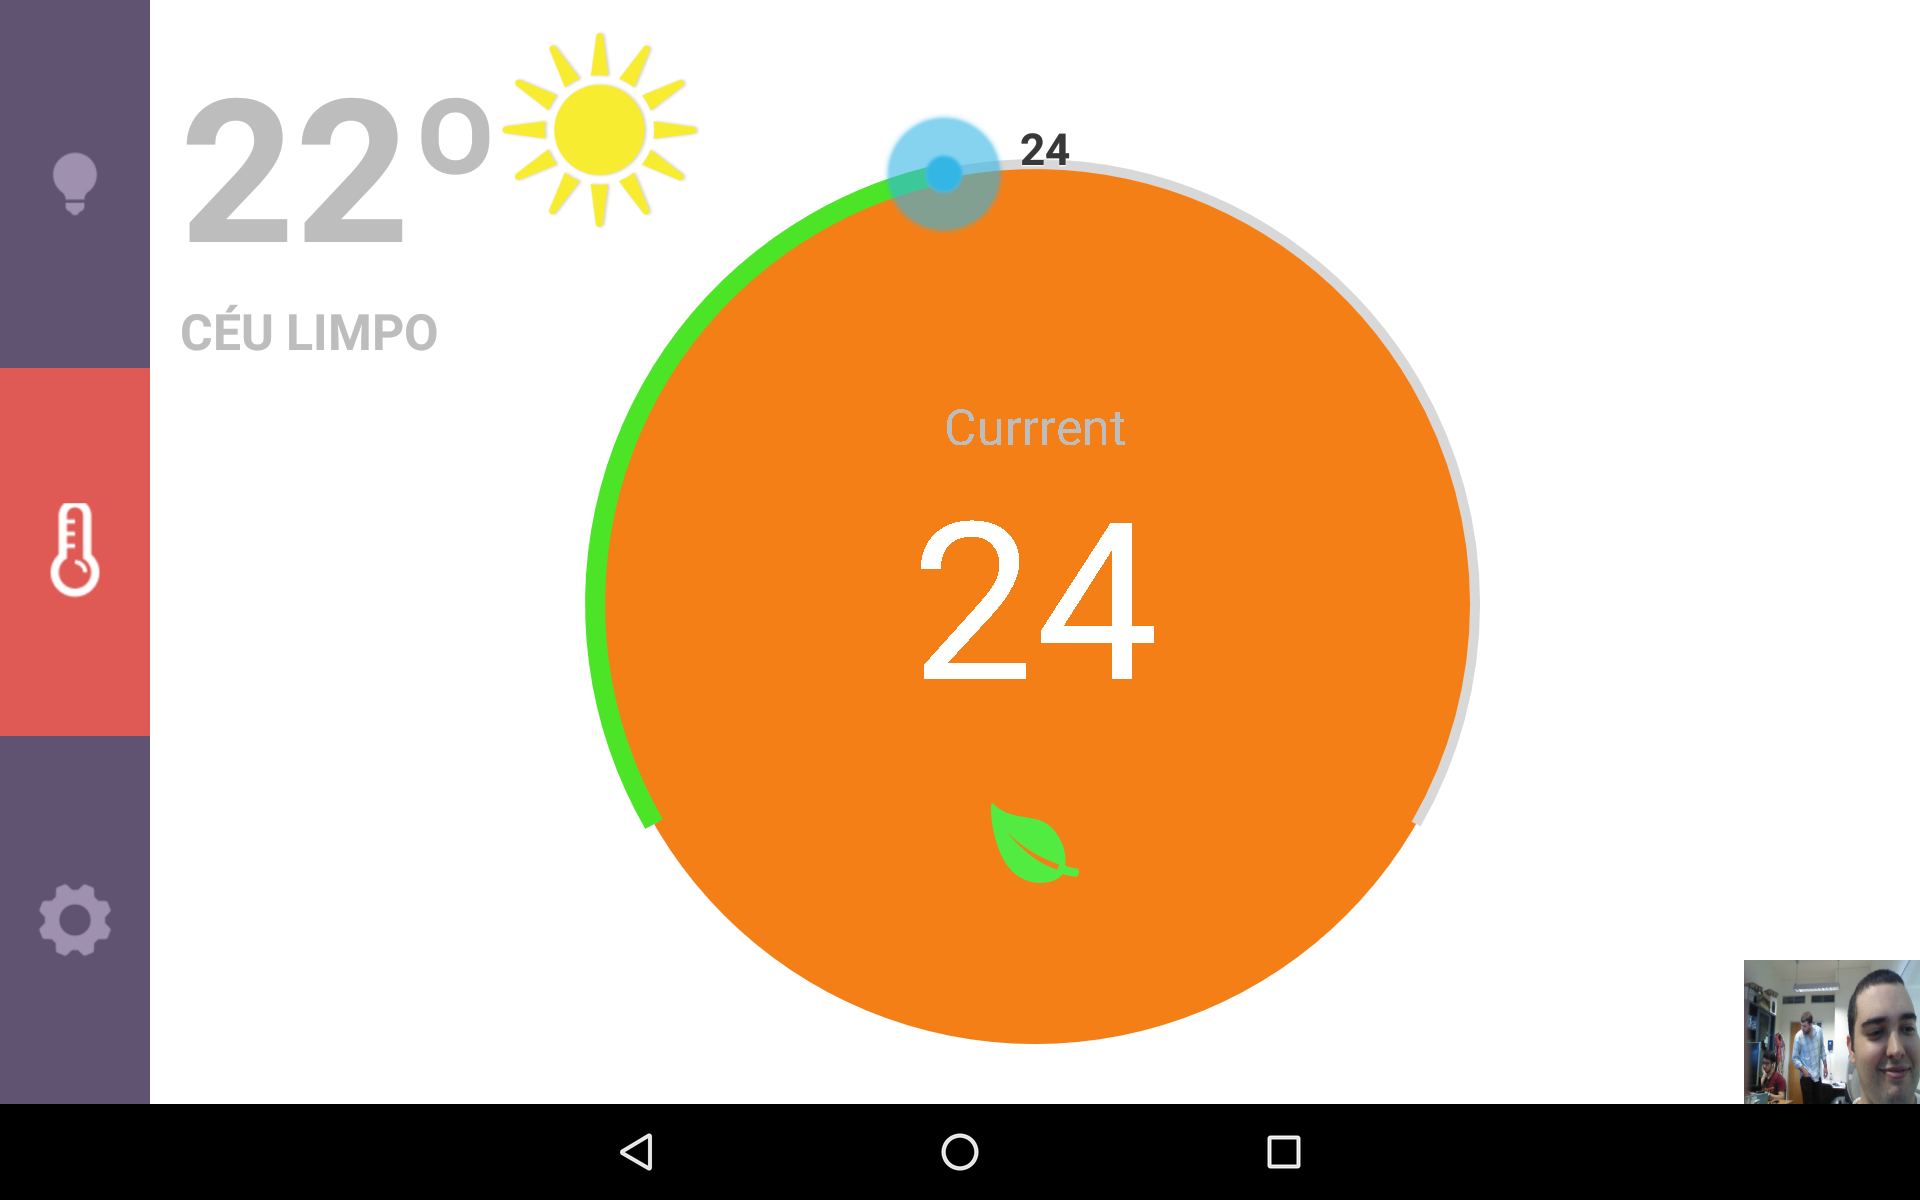
\includegraphics[width=0.7\textwidth]{Figures/screen_temperature}
\caption{Temperature screen.}
\label{screen_temperature}
\end{figure}



\begin{figure}[h]
\centering
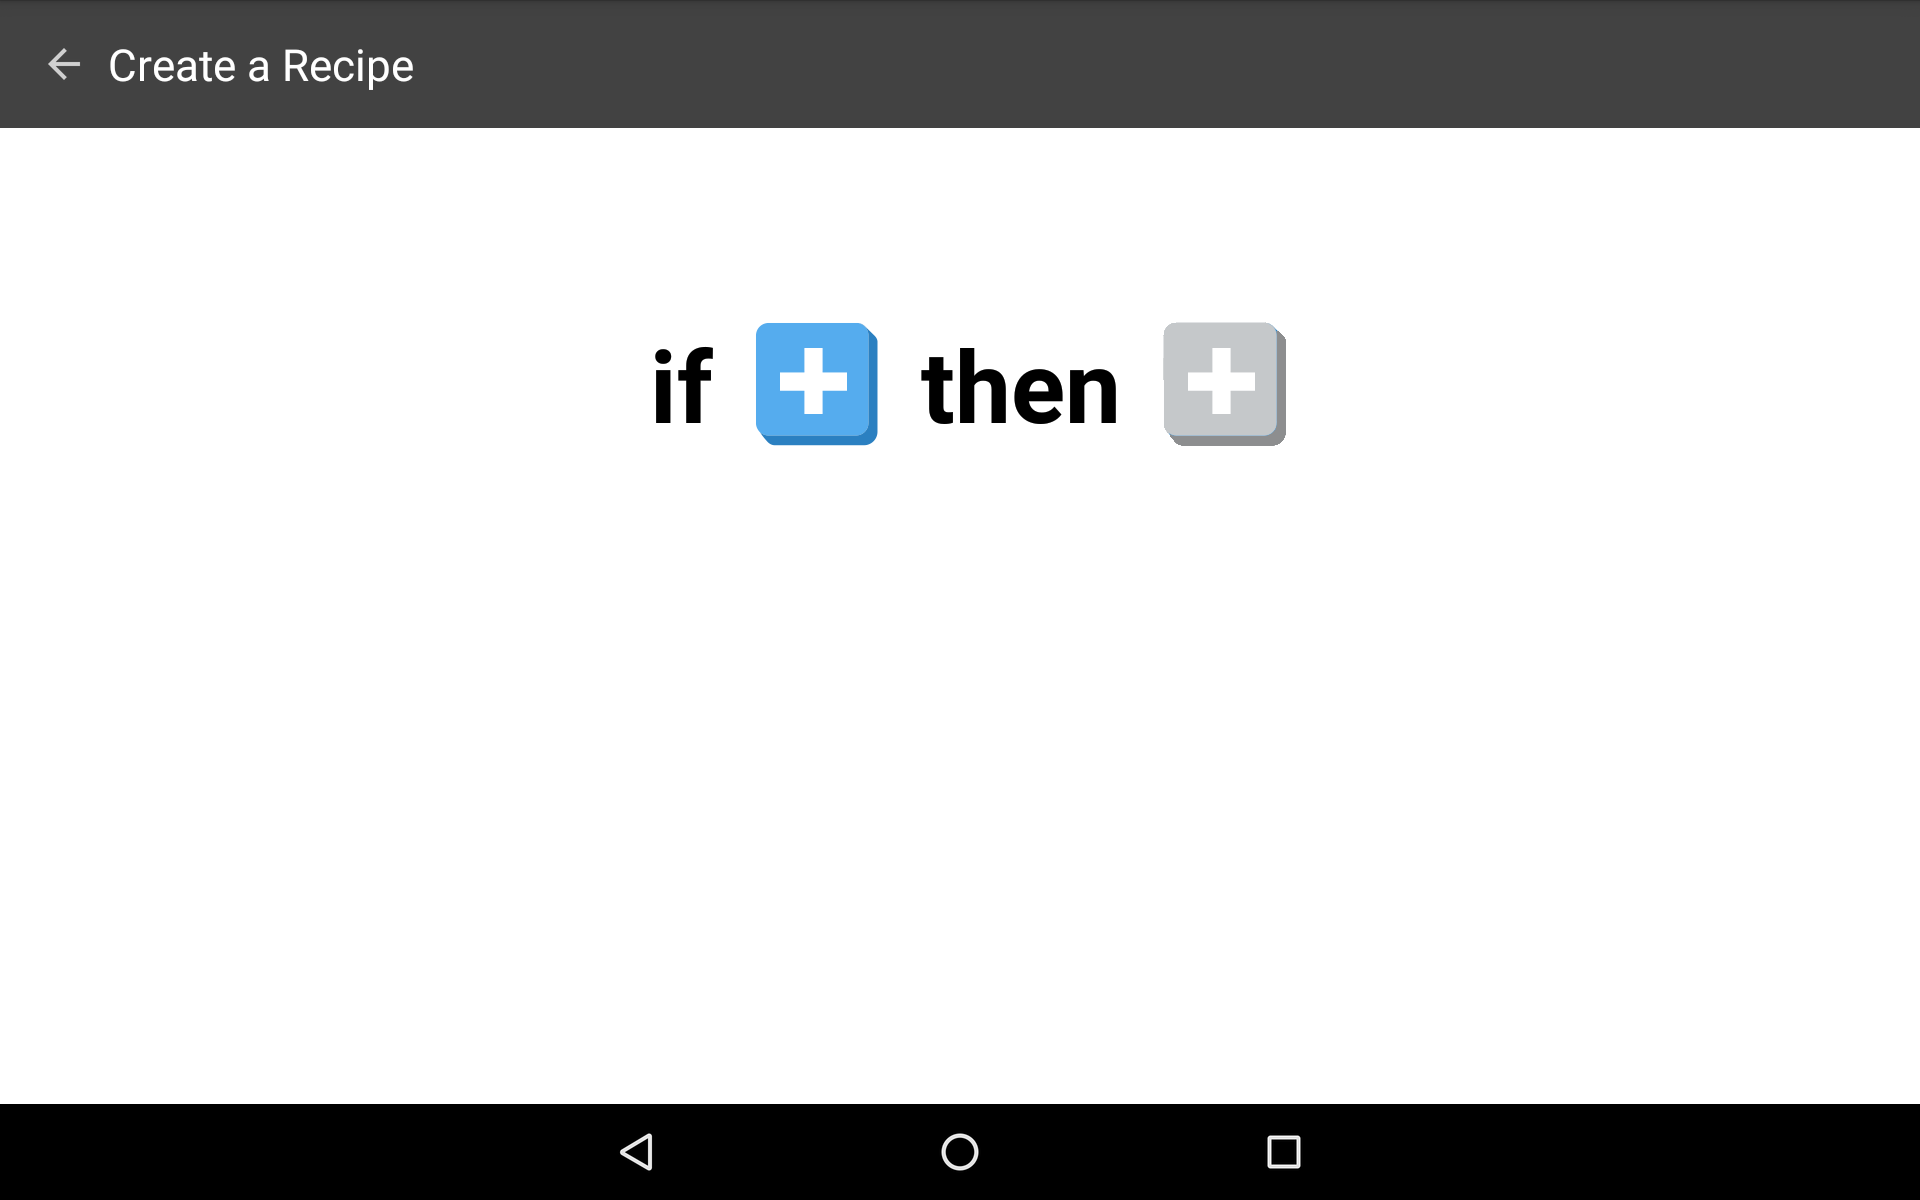
\includegraphics[width=0.7\textwidth]{Figures/create_recipe}
\caption{Temperature screen.}
\label{create_recipe}
\end{figure}

\begin{figure}[h]
\centering
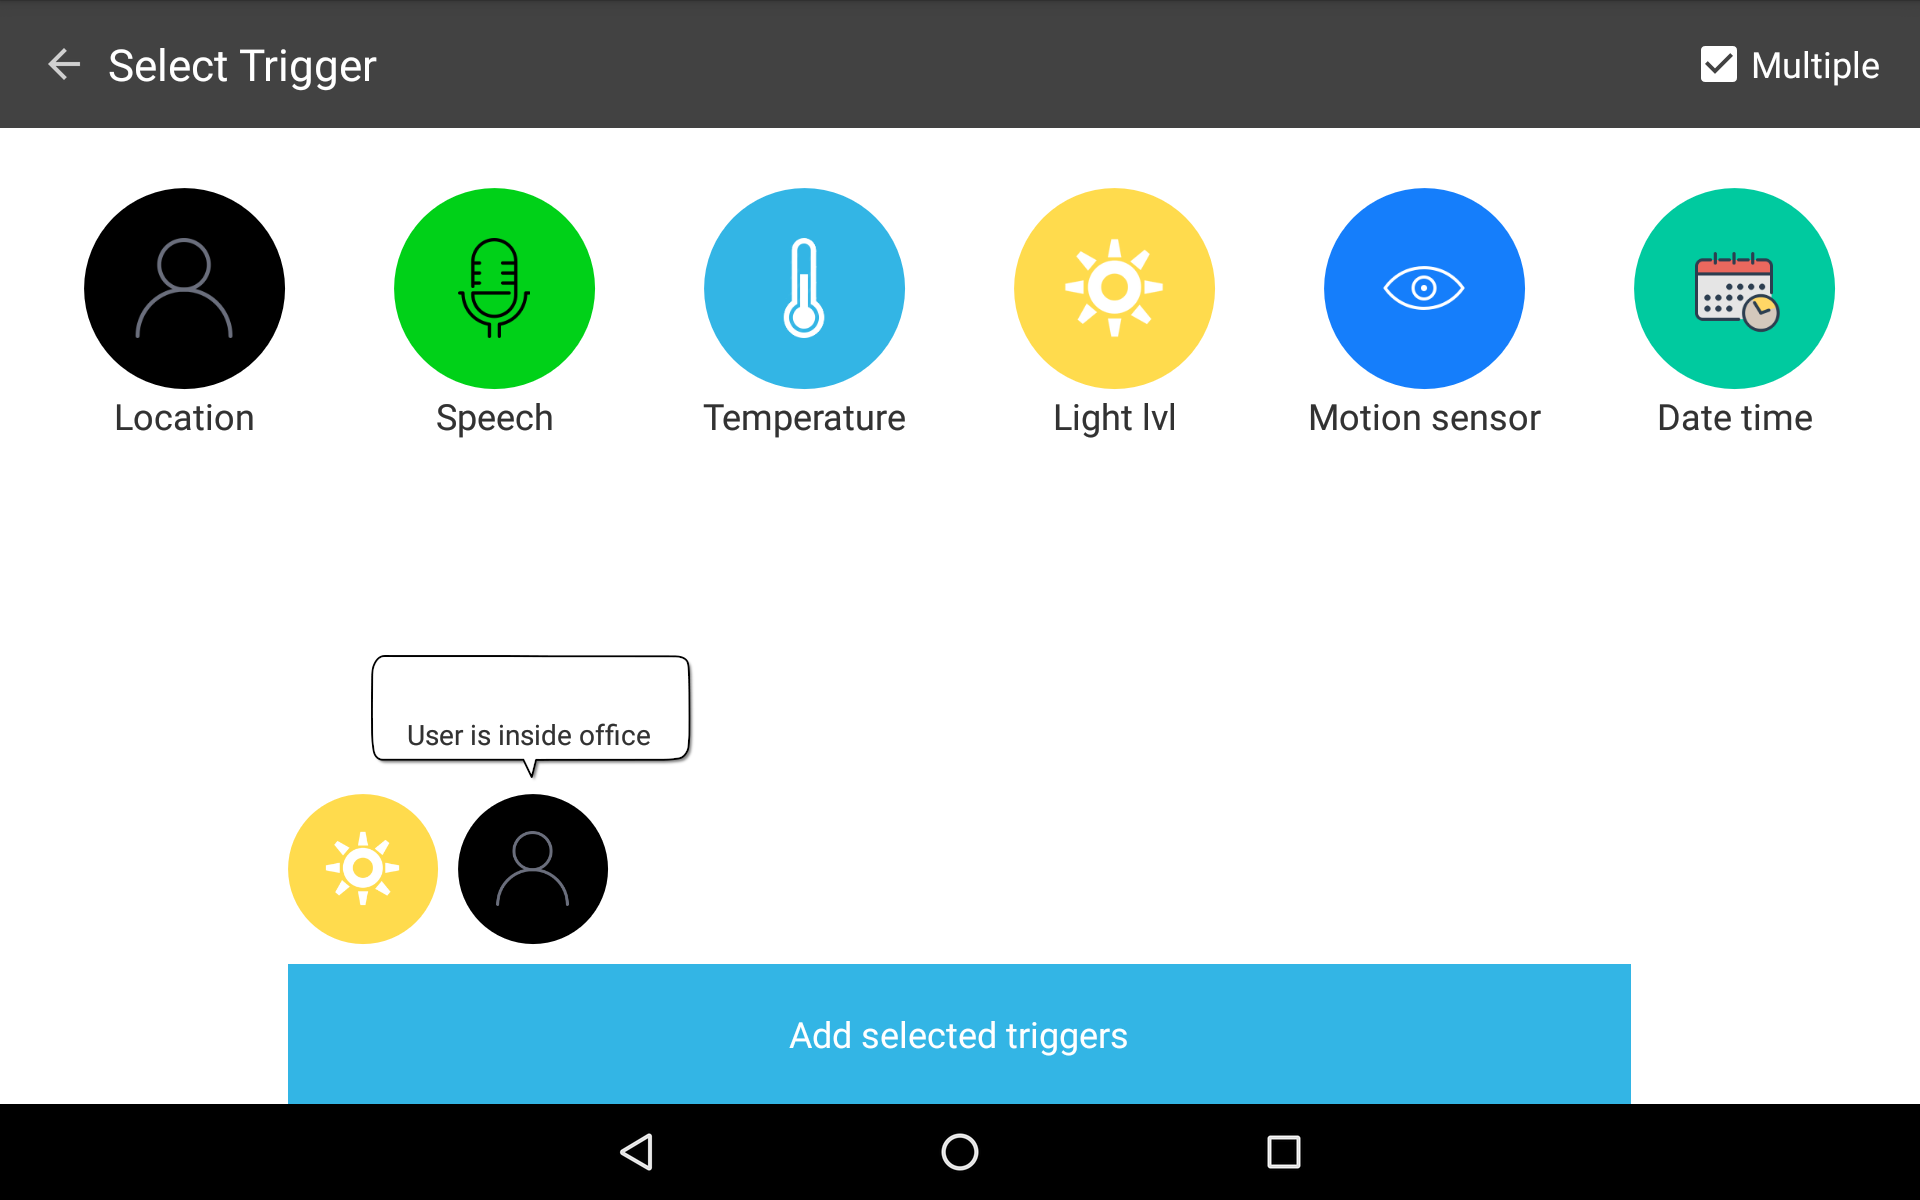
\includegraphics[width=0.7\textwidth]{Figures/screen_trigger}
\caption{Temperature screen.}
\label{screen_triggers}
\end{figure}

\begin{figure}[h]
\centering
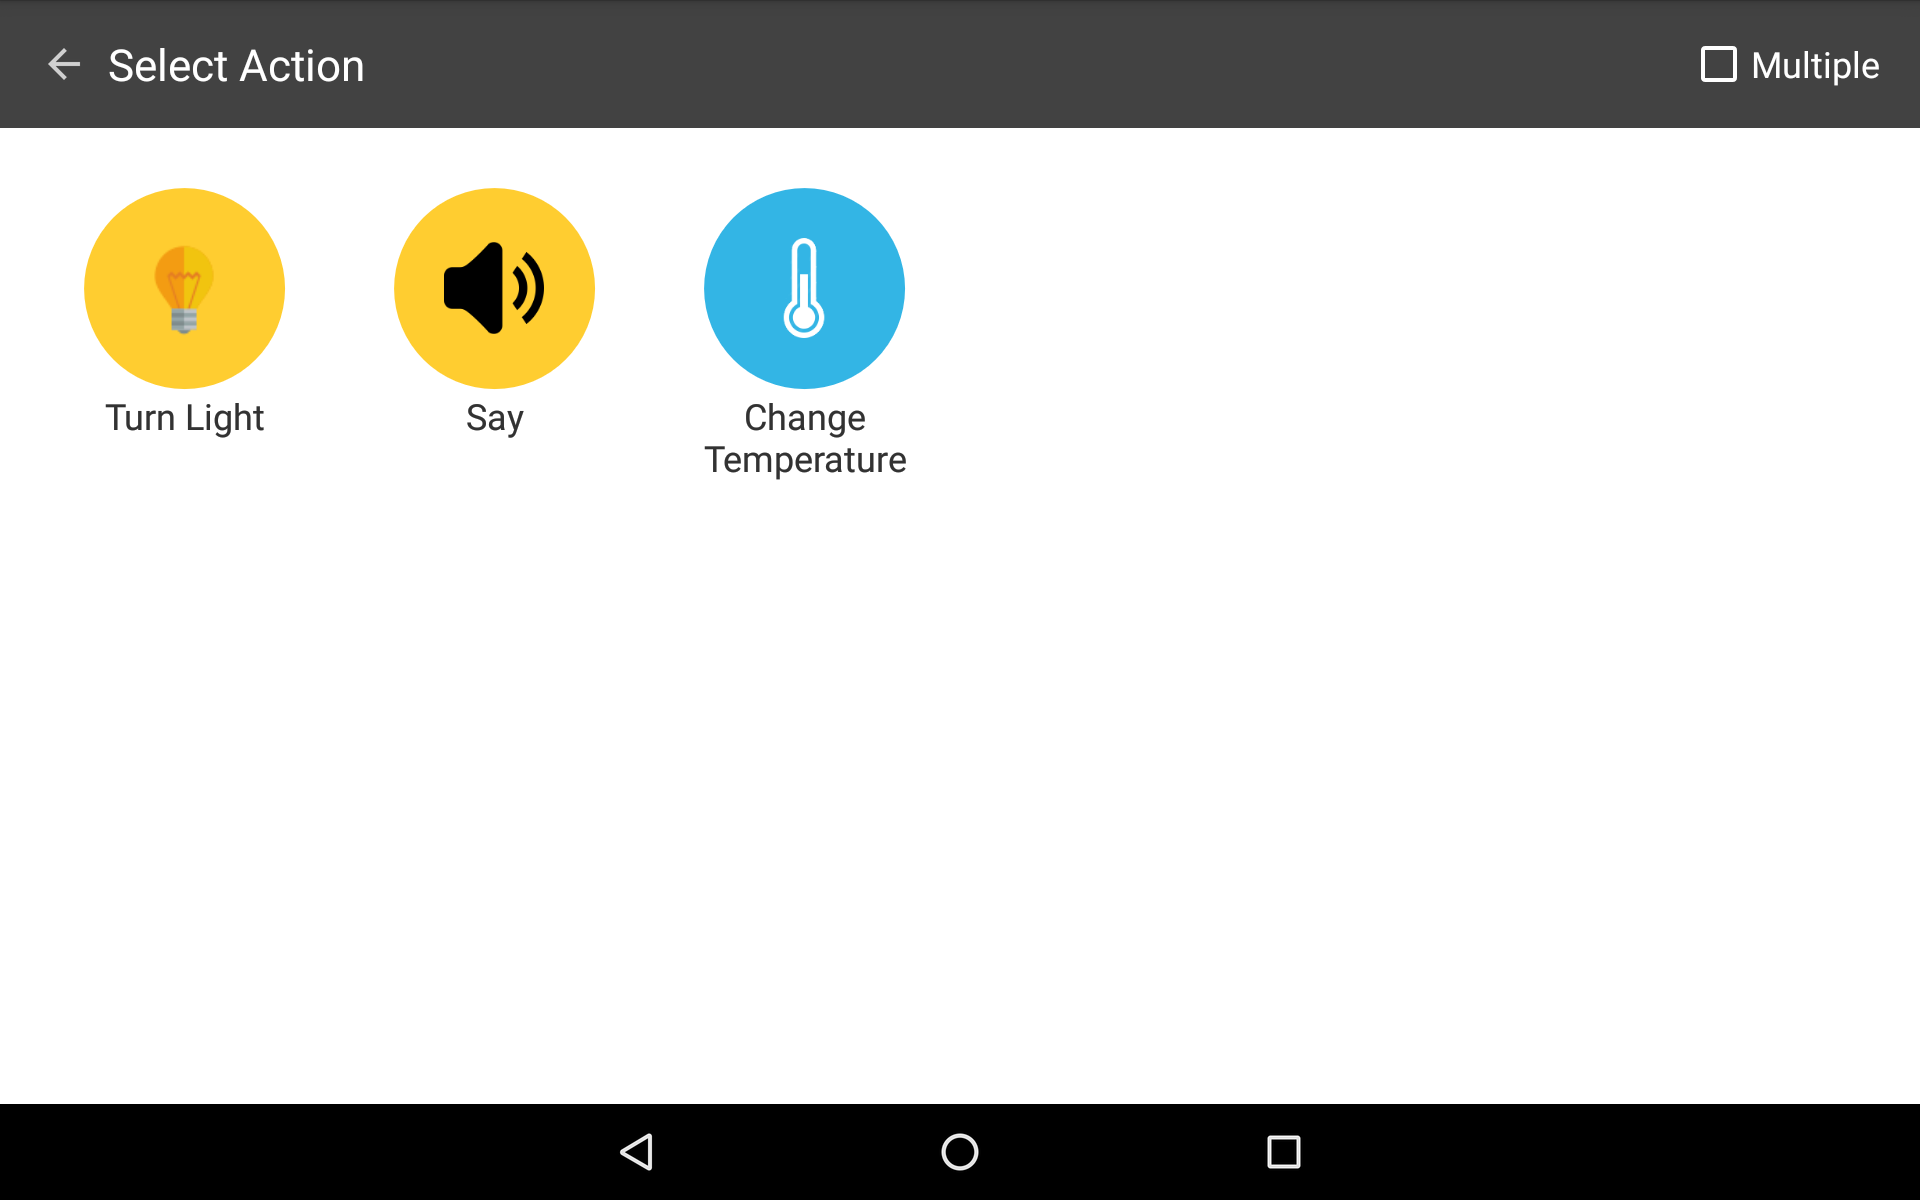
\includegraphics[width=0.7\textwidth]{Figures/screen_actions}
\caption{Temperature screen.}
\label{screen_actions}
\end{figure}

\begin{figure}[h]
\centering
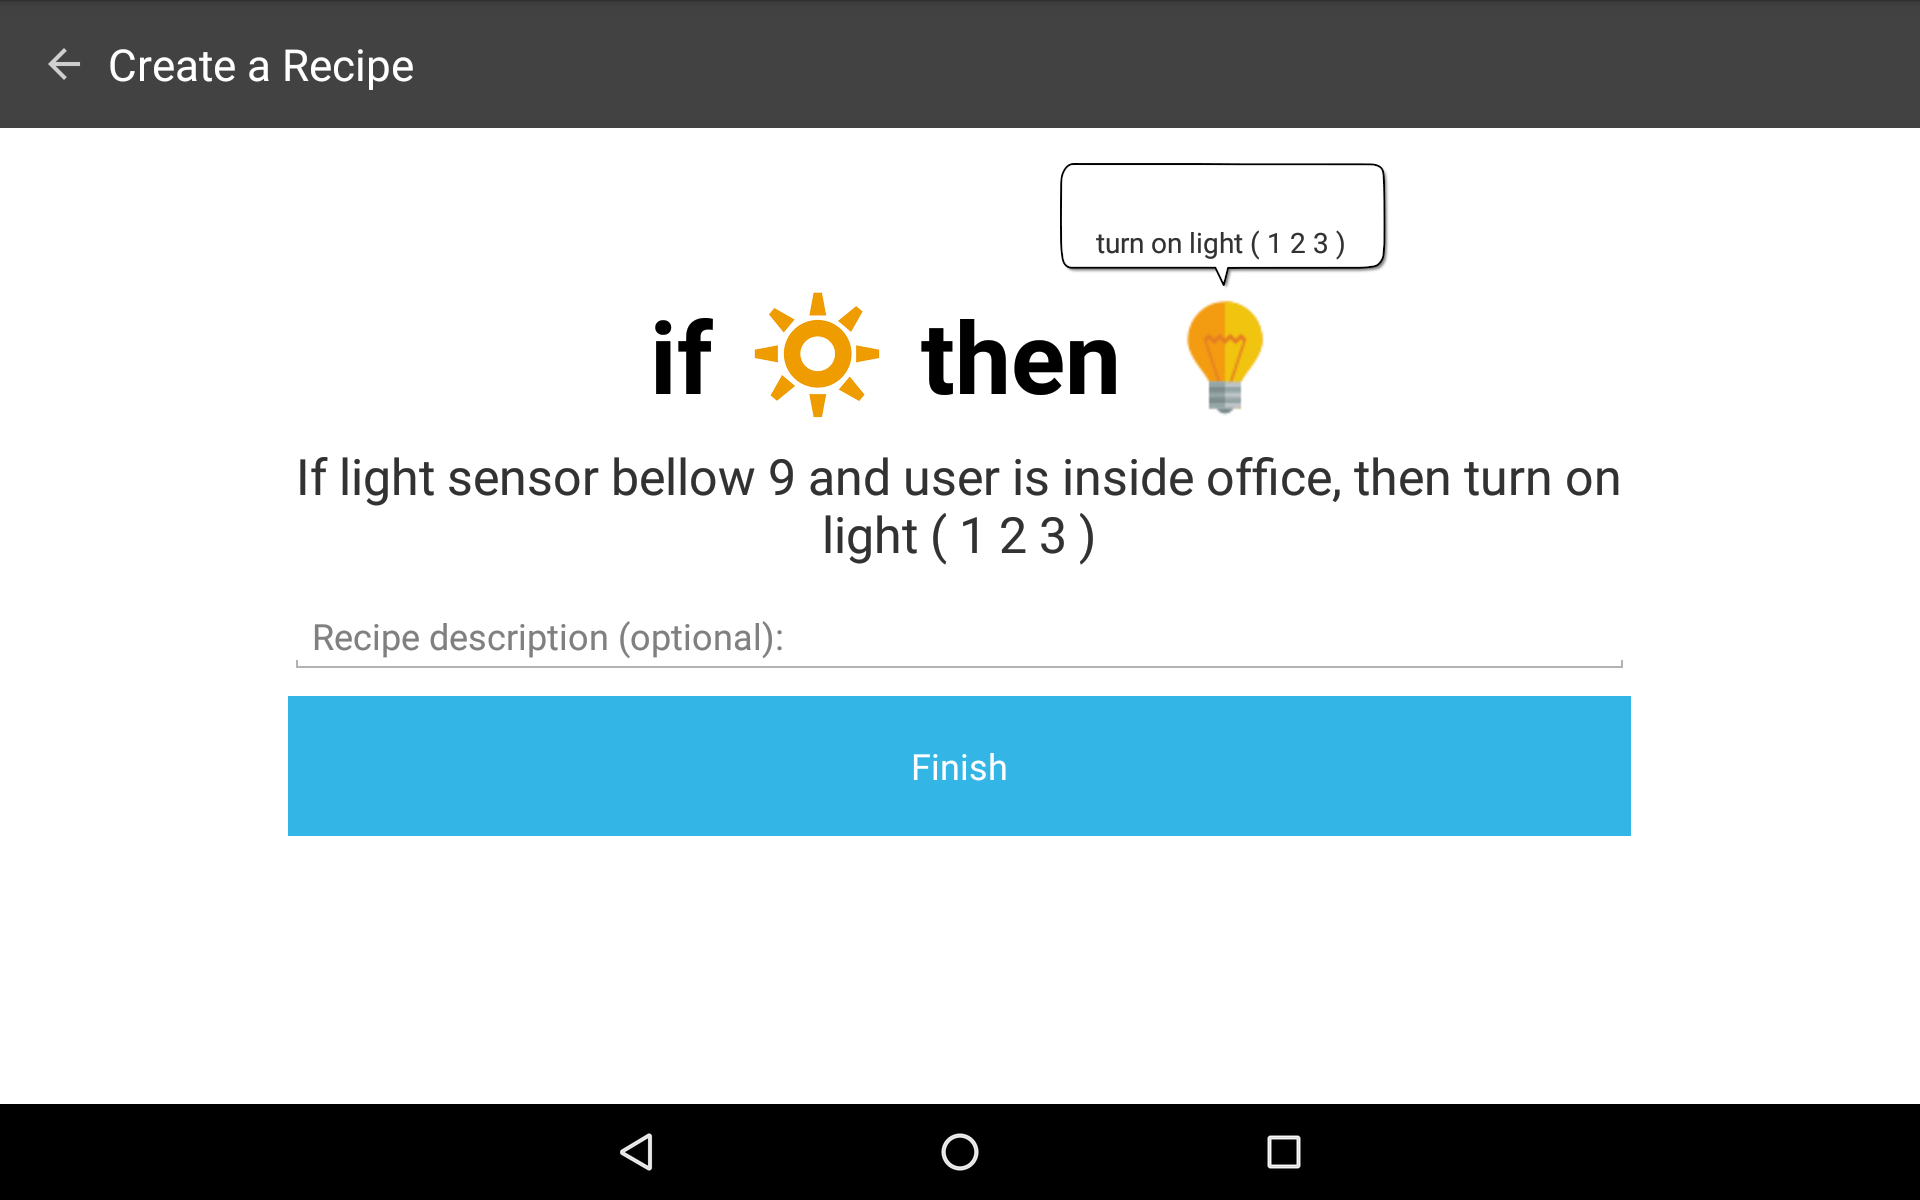
\includegraphics[width=0.7\textwidth]{Figures/screen_completed_recipe}
\caption{Temperature screen.}
\label{screen_completed_recipe}
\end{figure}


%\begin{figure}[h]
%\centering
%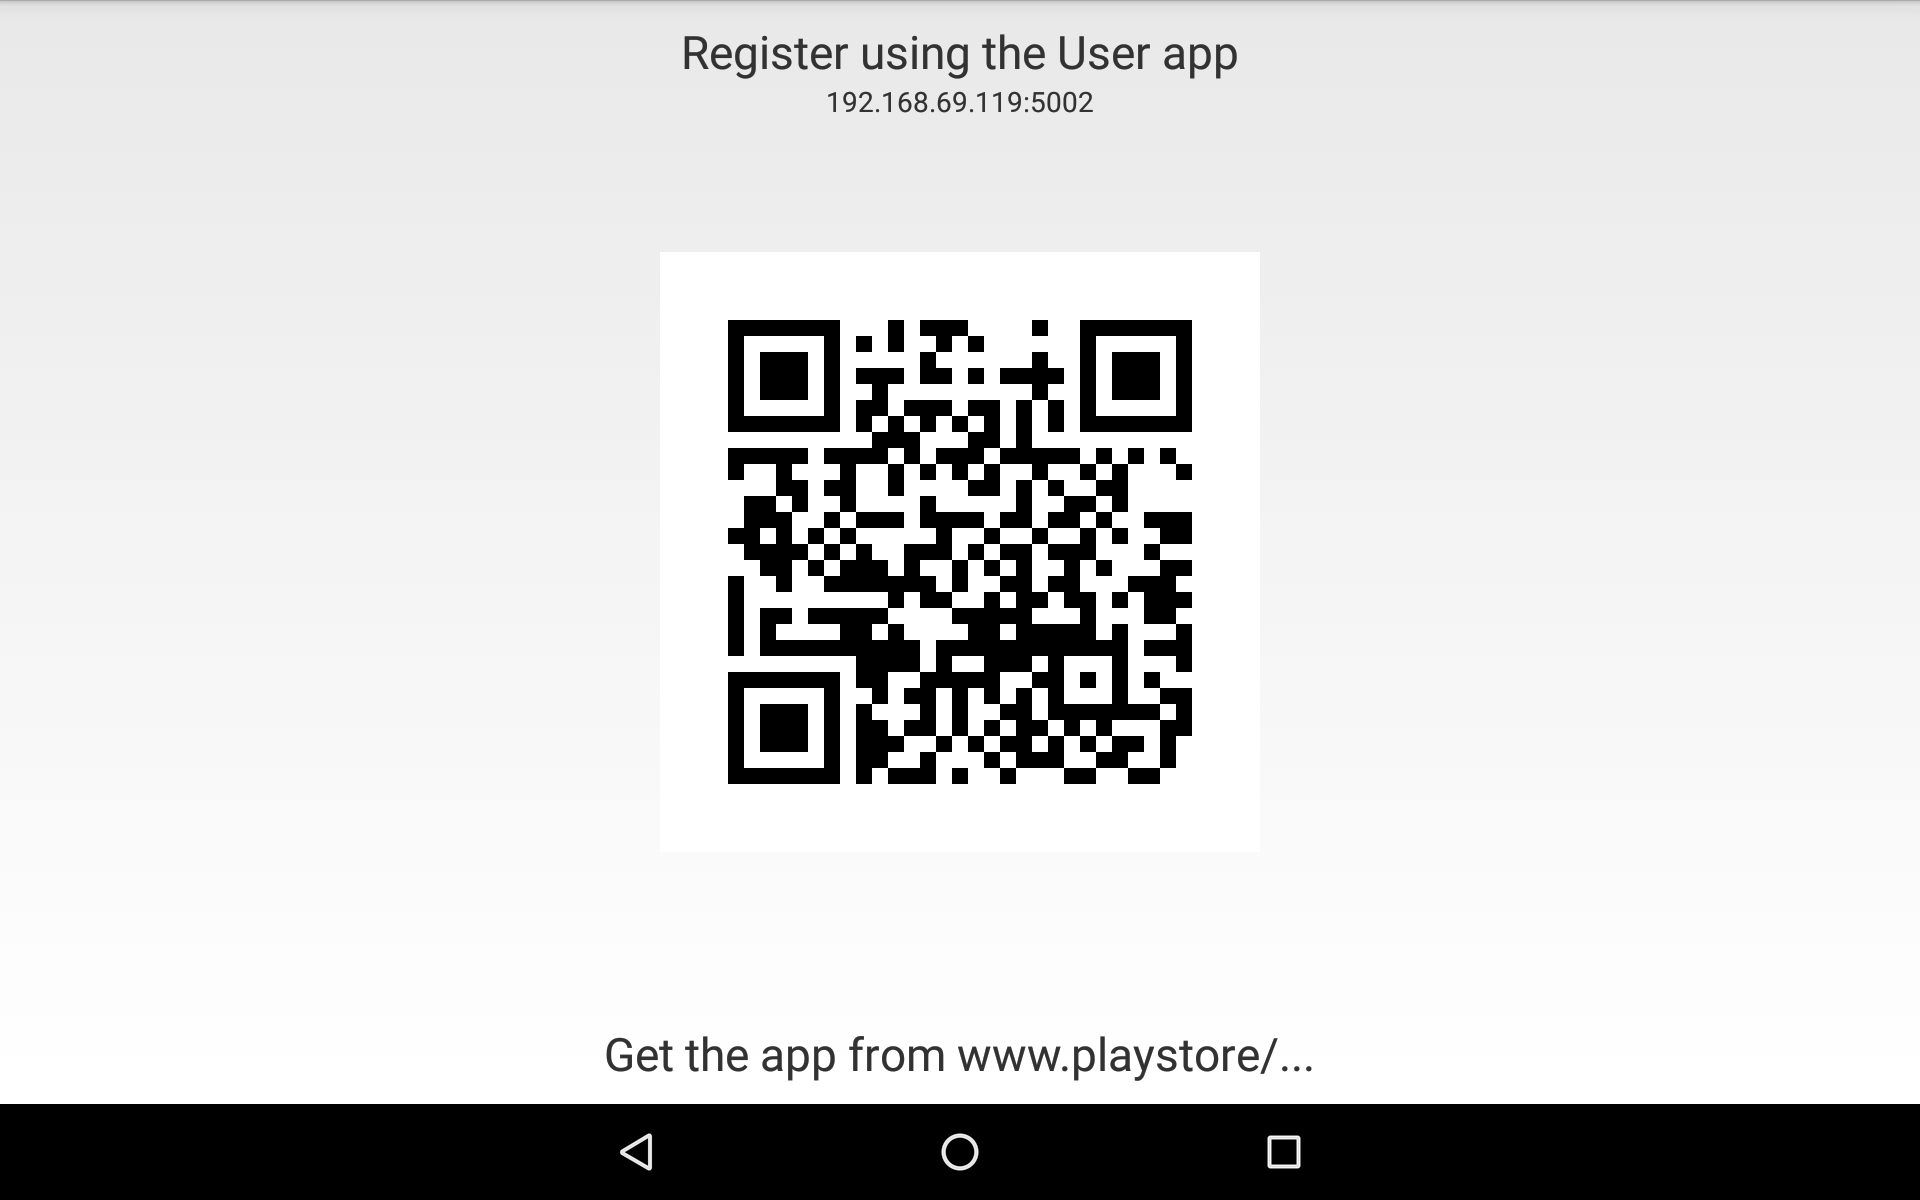
\includegraphics[width=0.7\textwidth]{Figures/screen_qr_code}
%\caption{Registration screen when using USER APP.}
%\label{screen_qr_code}
%\end{figure}


\subsection{USER APP}





if the user is inside the building (mobile app installed), it sends a message every 60 seconds. There is a timeout of 120 consecutive seconds, if no message is received in this time we assume the user has left the building.





